%prototype

The following chapter comprises the main activity of the project: the implementation of the TaWusel webservice and the TaWusel
Android application. At the beginning we take a look at the basic architecture design of the whole service in section
\ref{sec:GArc}. Afterwards the database design is described in a brief section.

\emptyRow
Subsequently to the fundamentals the section \ref{sec:Webs} takes a closer look at the implementation of the web service.

\emptyRow
Last but not least the focus of section \ref{sec:Andr} will be on the Android application. Here you will find a brief description
of its functions (see \ref{ssec:AndrDes}), some design thoughts regarding the class diagram and a description of the classes which
are used by the app (see \ref{ssec:AndrArc}) as well as an installation guide to run the app on your mobile device (see
\ref{ssec:AndrInst}). 

\emptyRow
You can retrieve more information if you follow the link to our issue tracker
(\url{https://github.com/nutztherookie/swp_kp2_2012_gruppe1/issues}) Here most of our task which came up while the implementation
are covered. There are also some issues which are labeled with the prefix "wishlist", these are suggestions how one could improve
the service in the future. The whole document with all estimated users stories can be found in appendix \ref{chp:US}.

\clearpage

\section{General architecture}\label{sec:GArc}
%general architecture
\begin{figure}[ht]
	\centering
	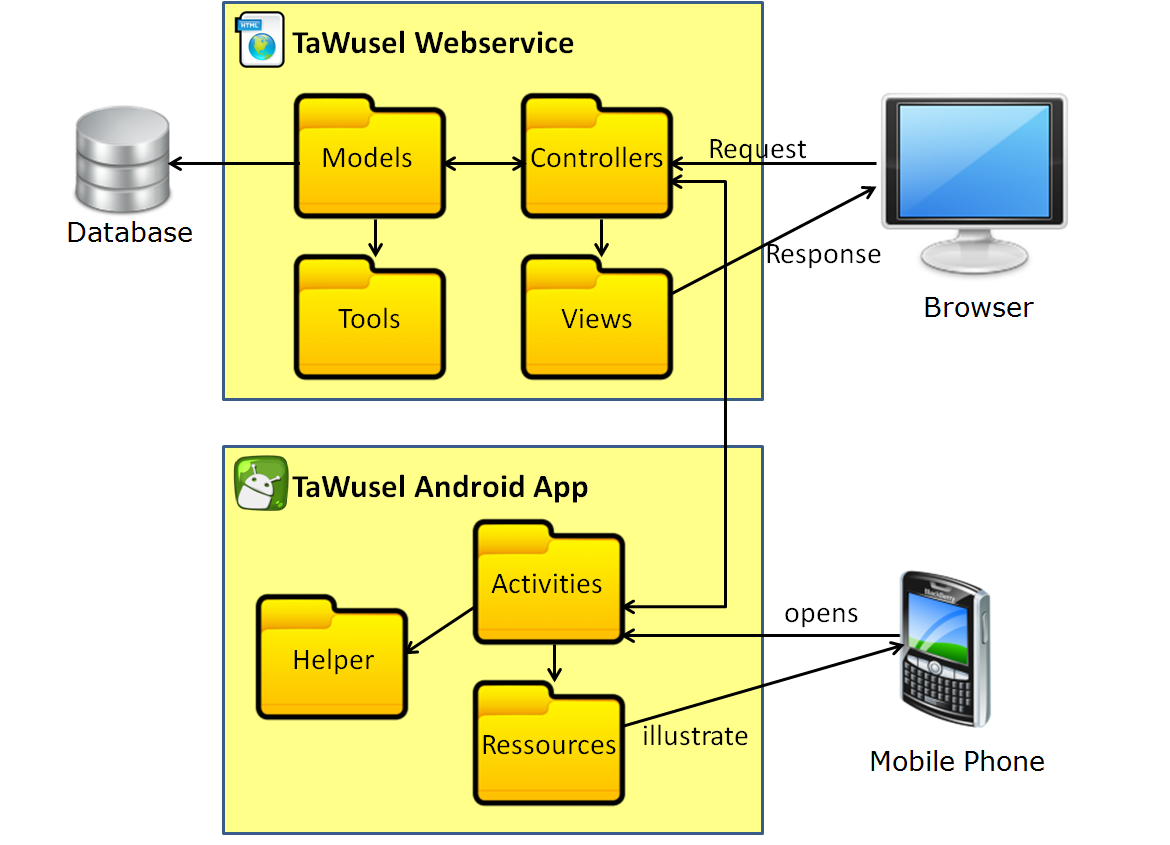
\includegraphics[width=0.8\textwidth]{images/Architekturdiagramm}
	\caption{architecture diagram}
	\label{img:Arch}
\end{figure}



\clearpage
\section{Database modeling}
%db modeling
\begin{figure}[ht]
	\centering
	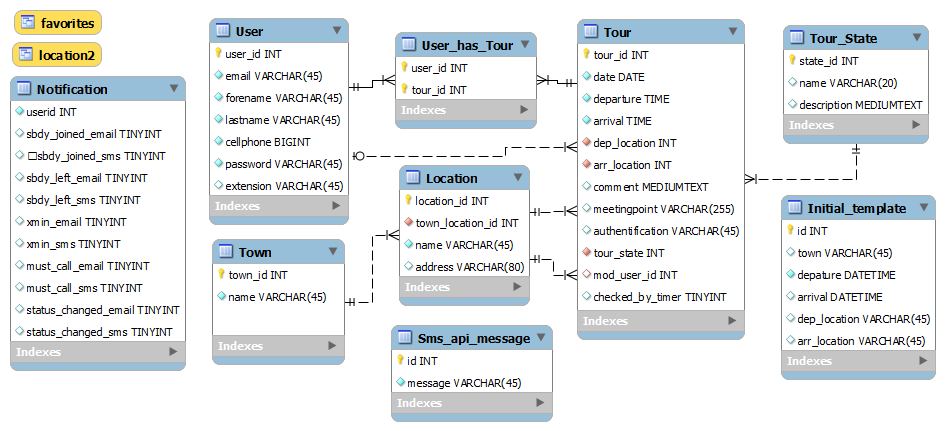
\includegraphics[width=0.8\textwidth]{images/Datenbank_Model}
	\caption{database model}
	\label{img:DBMod}
\end{figure}
Our database consists of a few tables for basic functionality, like user management or creation of a tour, and two views which
have to be used due to circumstances with play2 and its ANORM, which provides just some basic features and not the entire
capability of SQL.

\clearpage
\section{Webservice}\label{sec:Webs}
%webservice
\subsection{Description}\label{ssec:WedDesc}

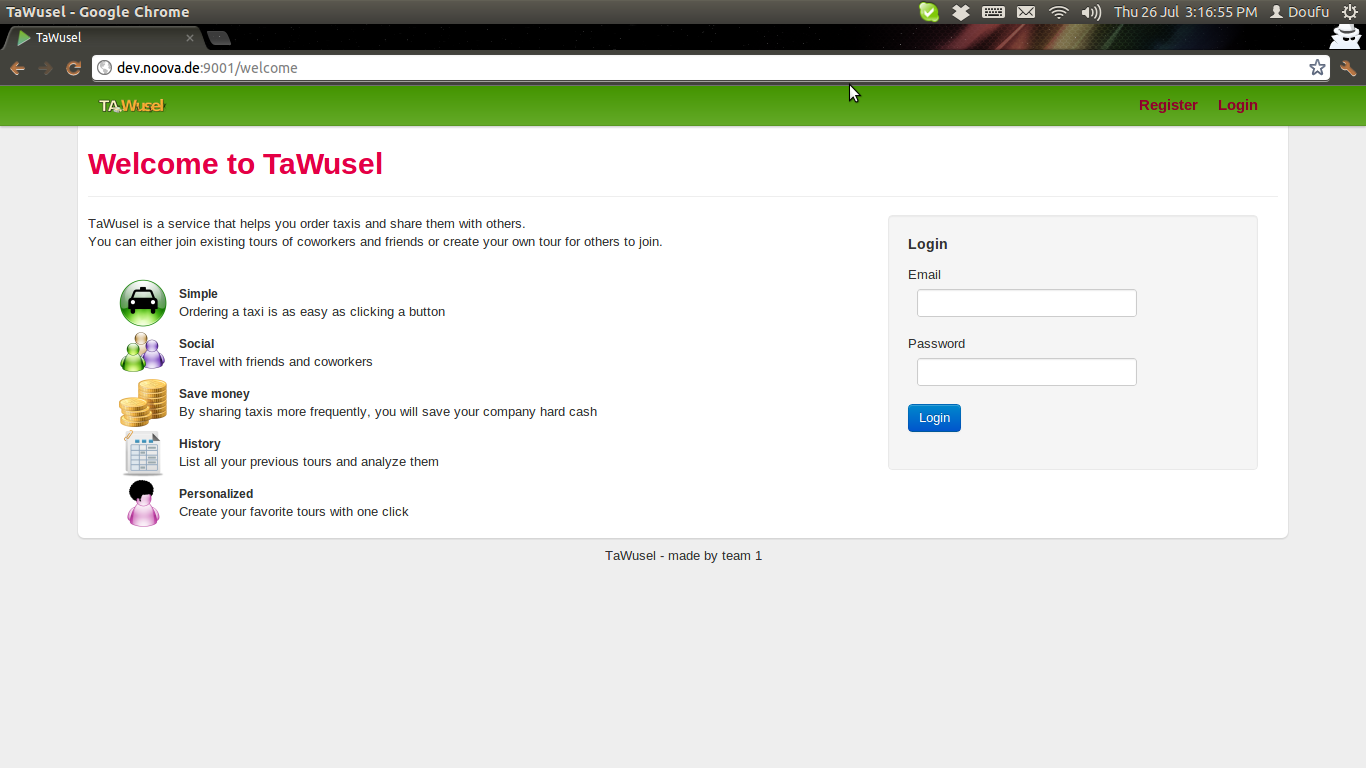
\includegraphics[width=16cm]{images/TaWusel_Web_Login.png}\label{img:WebLogin}
blabla


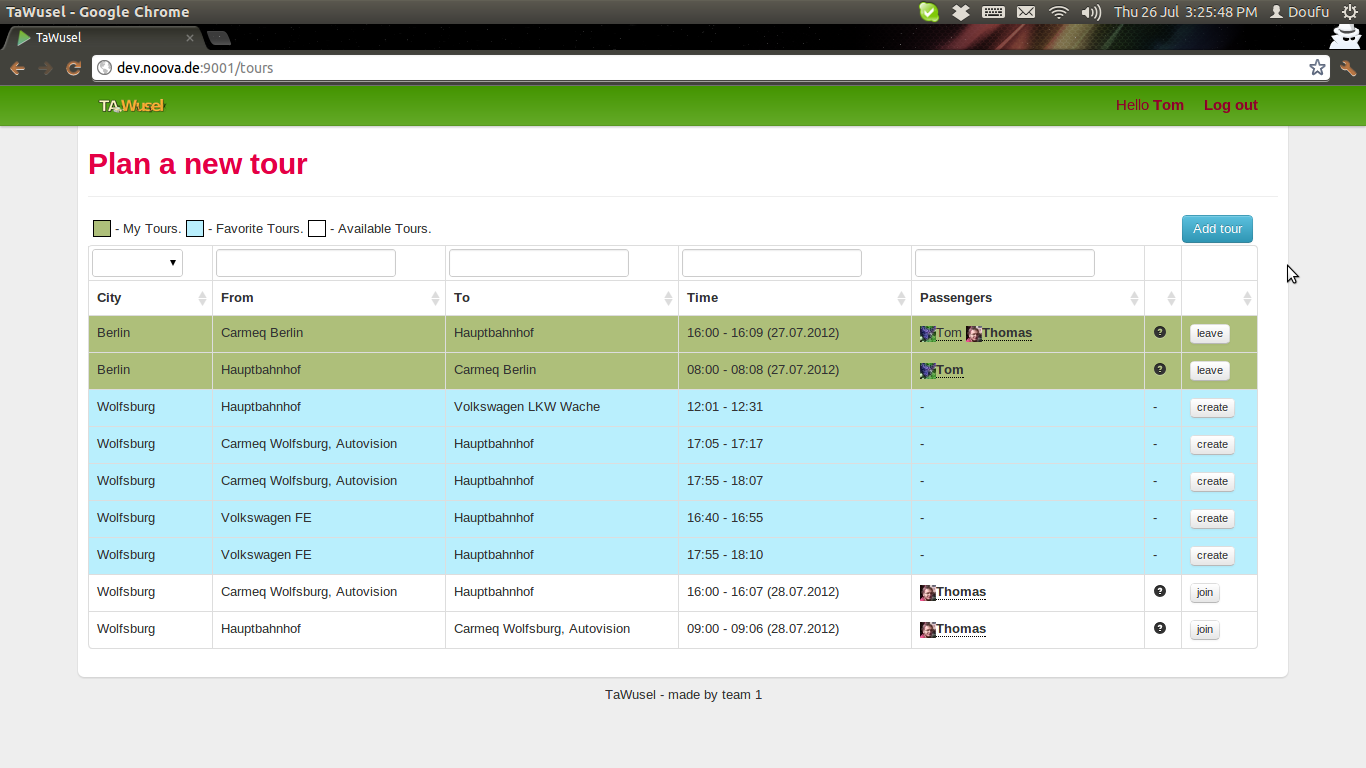
\includegraphics[width=16cm]{images/TaWusel_Web_main.png}\label{img:WebLogin}



\begin{figure}[h]
	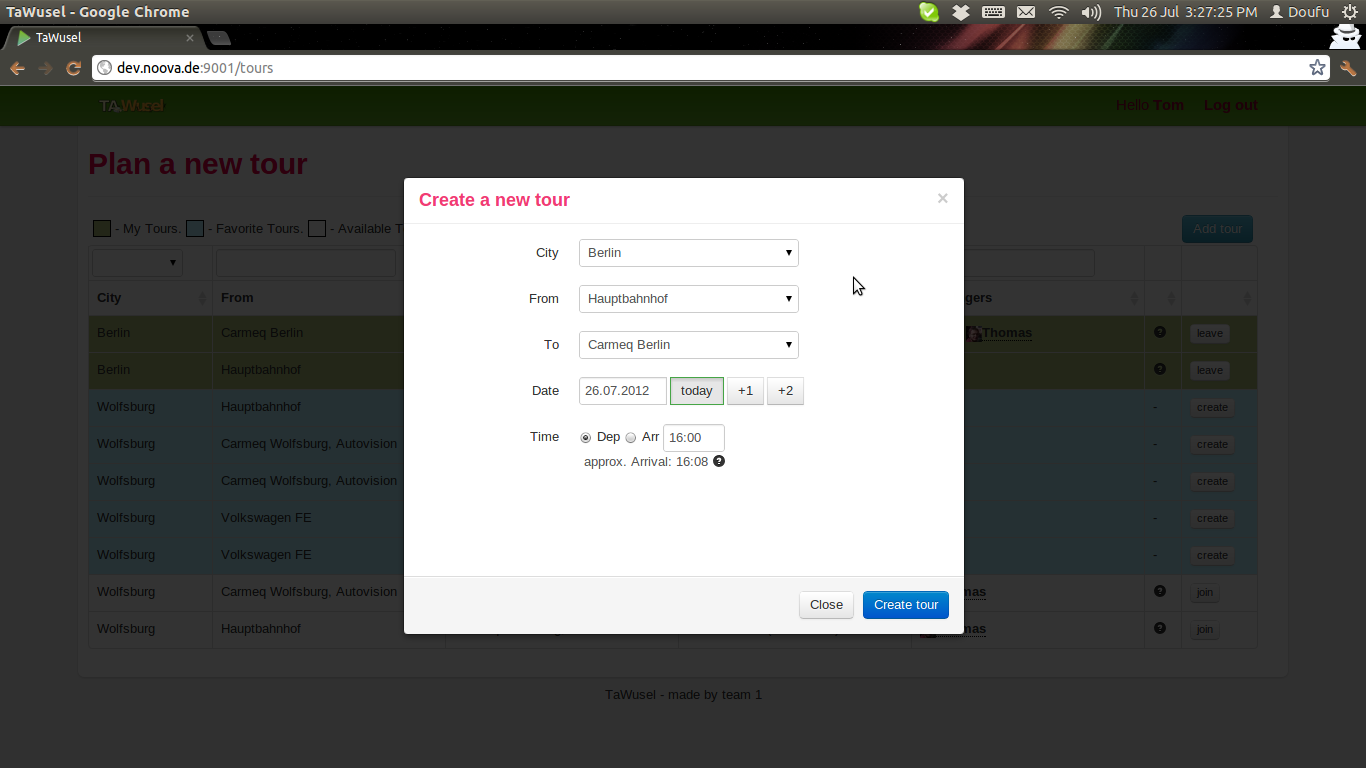
\includegraphics[width=16cm]{images/TaWusel_Web_create.png}
	\caption{modal panel for creating a tour}
	\label{img:WebLogin}
\end{figure}



\begin{figure}[h]
	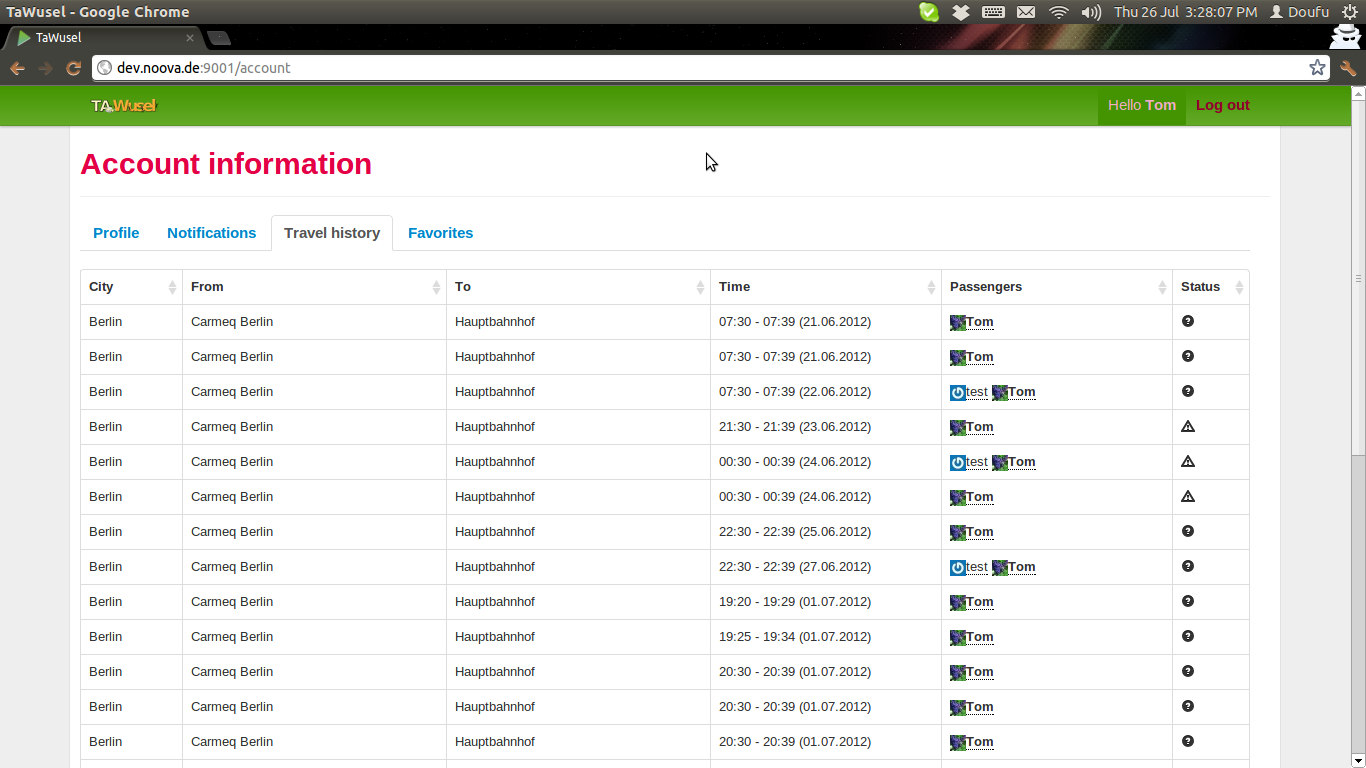
\includegraphics[width=16cm]{images/TaWusel_Web_history.png}
	\caption{profile page - history tab}
	\label{img:WebLogin}
\end{figure}
\subsection{Installation guide - Webservice}\label{ssec:WebInst}

The rough install instructions can also be found in the \texttt{INSTALL.md} file.
\begin{itemize}

\item As TaWusel uses the Play!2 framework (Scala version) obviously the first requirement is said framework. To obtain it, the
best way is to follow the official installation documentation from the Play!
website\footnote{\url{http://www.playframework.org/}}.

\item The next step is to set up a MySQL-database\footnote{In theory, other SQL-DBMS should work as well, since TaWusel uses
JDBC for its connections. However we have only used MySQL so far.} for your project.
As installing MySQL can obviously not be part of this documentation, we shall only briefly point towards the official
website\footnote{\url{http://dev.mysql.com/doc/refman/5.6/en/installing.html}} and name
XAMPP\footnote{\url{http://www.apachefriends.org/en/xampp.html}} and MAMP\footnote{\url{http://www.mamp.info}} as two easy
alternatives
for installing MySQL on Windows and Mac OS X respectively.\\
Example code for setting up the database:
\begin{verbatim}
CREATE DATABASE tawusel;
CREATE USER tawusel;
GRANT ALL ON tawusel.* TO tawusel@localhost IDENTIFIED BY 'pass';
\end{verbatim}
\small{To use other credentials, the \texttt{conf/application.conf} has to be changed accordingly.}

\item Lastly go to \url{https://github.com/nutztherookie/tawusel} and download TaWusel. Unzip, go to the project's root folder and
run \texttt{play run}.\\
Point your web browser to \url{http://localhost:9000/}


\end{itemize}

\clearpage
\section{Android App}\label{sec:Andr}
%android
\subsection{Description}\label{ssec:AndrDes}
\begin{floatingfigure}[r]{5cm}
	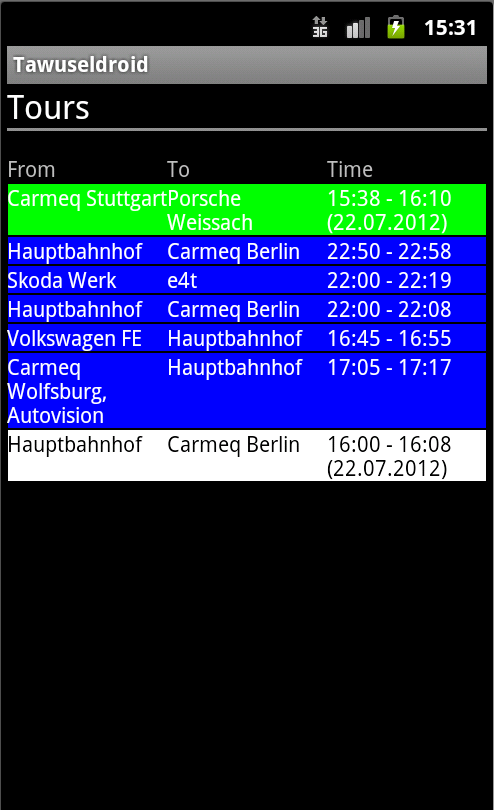
\includegraphics[width=4cm]{images/Tawuseldroid_tours.png}
	\caption{main view}
	\label{img:AndMV}
\end{floatingfigure}

\noindent
After the development of the key features of the TaWusel web service the team decided to implement an android app prototypically. This guarantees that all Carmeq employees who have access to an android phone can use the service more comfortable. The biggest advantage of an implementation of an android application is that the mobile phone doesn't need to have internet access at the whole time of the journey. On the other hand if one calls the web service with a web browser an internet connection is mandatory.

\emptyRow
The android application includes the most valuable features like creating a new tour or joining/leaving an existing tour. In figure \ref{img:AndMV} you can see the main view of the prototype. Like in the web service there is a table which is divided into three parts: the user's active tours, the templates to create a new to more comfortable and available tours created by other users. Since the application is a rough prototype the look and feel can be improved in most of the views, e.g. the colors of the tours table are just the standard android colors for green, blue and white to link their appearance to the corresponding entries in the web service.  

\emptyRow
\begin{floatingfigure}[l]{5cm}
	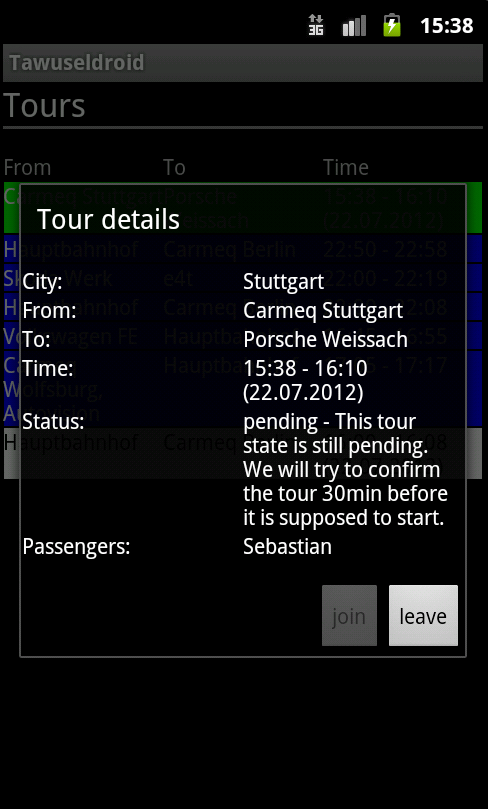
\includegraphics[width=4cm]{images/Tawuseldroid_details.png}
	\caption{details dialog}
	\label{img:AndDet}
\end{floatingfigure}
\noindent
By clicking on an existing tour a dialog is opened which shows more details according the chosen tour (see figure \ref{img:AndDet}). Here you find more information like the tour status or the passengers registered for it. For creating a new tour you can either pick a template (one of the blue rows) or click on the item "add tour" in the content menu. A dialog similar to the details dialog occurs. Here you can choose the city and the locations as well as the date and the time of the tour. To change the date as well as the departure or arrival time you just have to click on the corresponding field and a picker dialog appears.  A picture of the create dialog can be found in the appendix A in figure \ref{img:AndCD}.

\emptyRow
Unfortunately in the short period of development we were not able to implement a push function in the web service. So you have to fetch the tour data manually. For that reason just click on the item "update data" in the content menu. Remember that the mentioned activities call methods from the web service, therefore you need to have internet access.

\clearpage
\subsection{Architecture}\label{ssec:AndrArc}



\subsection{Installation guide}\label{ssec:AndrInst}

\begin{enumerate}
	\item Make sure you locate the tawusel.properties into the assets folder. Here you have to replace the json server property ("http://10.0.2.2:9000/") by the address of the server your tawusel service is running on.
	\item Generate your tawusel.apk. You can directly generate the apk from your eclipse project.
	\item Install the apk on your mobile phone.(Remark: the current version works stable on android 2.3.3 but its working on higher versions is not guaranteed)
\end{enumerate}


